\section{Game Architecture Overview}
% Diagram
% Beskriv diagram
% Hvorfor ikke class diagram 
% Details omkring diagram components er i module sections
Since we now have the architecture of Unity3D established, we can design the architecture of our game.
The diagram should have the essential systems described such that the development of the game can start immediately and we can quickly set up a playable version of the game.
The essential systems should support the requirements of the game which are described in section \ref{} \tododaniel{write requirements section of ref til den her}
\begin{itemize}
	\item Network to support multiplayer
	\item Input System which can support keyboard and mouse input, gamepad input, and touchscreen input.
	\item Level and mission generation which creates the game world and goal of the game, and can be easily modified by users
\end{itemize}
Early prototyping was done on the essential systems to find 3rd. party API's that would speed up the development of these systems.
With these main systems in mind we can set up the lower layer of the diagram.

\begin{figure}
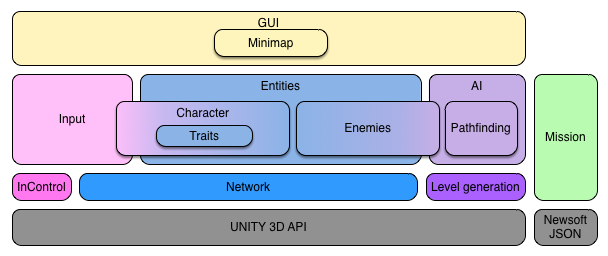
\includegraphics[width = \textwidth]{figures/architecture/game_architecture_overview.png}
\end{figure}

The network has to handle the enemies and characters in the game such that they can be synchronised with all the players, handled in the Entity structure above the network level. 
Furthermore, these characters should be connected to the input system as they are to be controlled by players.

Enemies are not controlled by players but are AI's in the game and have a specific behaviour.
The way they are moving throughout the map should be controlled by some AI system which is created from the input of the level generator.
